\documentclass[11pt,oneside,letterpaper]{article}

% graphicx package, useful for including eps and pdf graphics
\usepackage{graphicx}
\usepackage{grffile}
%\DeclareGraphicsExtensions{.pdf,.png,.jpg}

% basic packages
\usepackage{color} 
\usepackage{parskip}
\usepackage{float}


% reference figures across documents
\usepackage{xr}
\externaldocument{mers-structure_supp}

% text layout
\usepackage{geometry}
\geometry{textwidth=15cm} % 15.25cm for single-space, 16.25cm for double-space
\geometry{textheight=22cm} % 22cm for single-space, 22.5cm for double-space

% helps to keep figures from being orphaned on a page by themselves
\renewcommand{\topfraction}{0.85}
\renewcommand{\textfraction}{0.1}

% bold the 'Figure #' in the caption and separate it with a period
% Captions will be left justified
\usepackage[labelfont=bf,labelsep=period,font=small]{caption}

% review layout with double-spacing
%\usepackage{setspace} 
%\doublespacing
%\captionsetup{labelfont=bf,labelsep=period,font=doublespacing}

% cite package, to clean up citations in the main text. Do not remove.
%\usepackage{cite}
\usepackage{natbib}
%\renewcommand\citepleft{(}
%\renewcommand\citepright{)}
%\renewcommand\citepform[1]{\textsl{#1}}

\usepackage{amsmath}

% Remove brackets from numbering in list of References
%\renewcommand\refname{\large References}
%\makeatletter
%\renewcommand{\@biblabel}[1]{\quad#1.}
%\makeatother

\usepackage{authblk}
\renewcommand\Authands{ \& }
\renewcommand\Authfont{\normalsize \bf}
\renewcommand\Affilfont{\small \normalfont}
\makeatletter
\renewcommand\AB@affilsepx{, \protect\Affilfont}
\makeatother

% comments
\usepackage{ulem}
\definecolor{purple}{rgb}{0.459,0.109,0.538}
\def\tb#1#2{\sout{#1} \textcolor{purple}{#2}} 
\def\tbc#1{\textcolor{purple}{[#1]}}

% symbols
\newcommand{\chiSq}{\chi^{2}_{df}}
\newcommand{\dtmrca}{\Delta_\mathrm{TMRCA}}
\newcommand{\undtmrca}{\delta_\mathrm{TMRCA}}
\newcommand{\dspr}{d_\mathrm{SPR}}

%%% TITLE %%%
\title{\vspace{1.0cm} \LARGE \bf MERS structure}

\author[1]{Gytis Dudas}
\author[2]{Luiz Max Carvalho}
\author[1]{Allison Black}
\author[1]{Trevor Bedford}
\author[2,4,5]{Andrew Rambaut}

\affil[1]{Vaccine and Infectious Disease Division, Fred Hutchinson Cancer Research Center, Seattle, WA, USA}
\affil[2]{Institute of Evolutionary Biology, University of Edinburgh, Edinburgh, UK}
\affil[4]{Fogarty International Center, National Institutes of Health, Bethesda, MD, USA}
\affil[5]{Centre for Immunology, Infection and Evolution at the University of Edinburgh, Edinburgh, UK}

\date{\today}

\begin{document}
\maketitle

\begin{abstract}

Middle East Respiratory Syndrome coronavirus (MERS-CoV) is a zoonotic virus causing significant mortality and morbidity largely in the Arabian Peninsula.
The epidemiology of the virus is relatively poorly understood with most MERS patients being older males with comorbidities, although large nosocomial have occurred, notably in Jeddah, Riyadh and South Korea.
Our understanding of MERS-CoV epidemiology is further complicated by some patients not recalling contact with camels, the accepted reservoir for MERS-CoV, or any other livestock, suggesting significant cryptic MERS-CoV circulation in communities.
Seroepidemiology has been employed extensively during the time since the discovery of MERS-CoV to understand the exposure and therefore risk among camels and humans alike, but various sequencing efforts have not been fully leveraged against this zoonotic virus.
Here we use existing MERS-CoV sequencing data to estimate the number of times the virus has been introduced into humans and use the distribution of sequence clusters to estimate the reproductive number for the virus from sequence data alone.
We confirm that MERS-CoV has relatively poor capacity to spread in humans and arrive at an estimate of at least 65 zoonotic introductions of the virus into humans.

\end{abstract}

\pagebreak

\section*{Introduction}
Middle East Respiratory Syndrome Coronavirus (MERS-CoV) is a zoonotic infection of humans in the Arabian Peninsula originating from camels.
The virus, first discovered in 2012 \cite{WHO_2016}, has gone on to cause more than 1800 infections with at least 600 associated deaths.
Its epidemiology remains obscure, largely because outbreaks are observed among the most severely affected patients, such as older males with comorbidities.
Whilst contact with camels is often reported by patients, many do not recall contact with any livestock, suggesting a significant but unobserved community contribution to the outbreak.
Studies into MERS-CoV epidemiology often rely on serology to identify factors associated with MERS CoV exposure in potential risk groups or hosts.
The new era of genomic epidemiology, however, has repeatedly shown the utility of sequence data in outbreak scenarios.
Often only sequence data can pinpoint sources of pathogens and discriminate between multiple and single source scenarios, which are a fundamental part of quantifying risk.
Sequencing MERS-CoV has been performed as part of initial attempts to link human infections with the camel reservoir, nosocomial outbreak investigations and routine surveillance.

It is accepted that human MERS-CoV infections are a result of multiple introductions of the virus into humans, but no study has attempted to go beyond educated guesses about this number.
Here we use existing MERS-CoV sequence data to investigate the population structure of the virus between two of its known hosts: humans and camels.
By explicitly modelling the evolution of MERS-CoV between these two distinct host populations we show that human MERS infections are the result of frequent and unidirectional spillover events from camels into humans.
Inter-outbreak evolution of the virus occurs exclusively in camels, highlighting the need for genomic surveillance of MERS-CoV in the reservoir as well.
We also use the sequence clusters recovered from our population structure analyses to estimate the reproductive number for the virus (R$_{0}$), which is in agreement with previous findings that MERS-CoV is, on average, poor at spreading in human populations.
Our analyses also capture seasonal variation in zoonotic transmission patterns, with indications that particularly large outbreaks are the result of zoonotic transmissions that take place at the beginning of each new year.


%Here we use 307 largely complete MERS-CoV genomes, 91 of which are from camel viruses, to explicitly model the population structure of the virus in humans and camels in order to arrive at an estimate of the number of times the virus has been introduced into human populations.
%We then explore the resulting sequence clusters that can be thought of as replicates of the transmission process, albeit with different settings, as the data include large nosocomial outbreaks.

%\begin{figure}[h]
% \centering		
%	\includegraphics[width=0.45\textwidth]{figures/}
%	\caption{\textbf{}
%	
%	}
%	\label{}
%\end{figure}

\section*{Results}

\subsection*{Recombination occurs in the reservoir}
Recombination has been shown to occur in all genera of coronaviruses, including MERS-CoV.
Since detectable and problematic recombination in RNA viruses requires co-infection with distinct viral genotypes humans were ruled out as a suitable recombination environment \textit{a priori}.
Here we confirm this assumption by showing that evolution of MERS-CoV within human clusters is clonal.
This is not surprising, since zoonotic transmission of MERS-CoV into humans is relatively rare, of limited diversity at the point of introduction and viral diversity in humans is ultimately transient.
All of these factors act to make co-infection of humans with MERS-CoV exceedingly rare.
It is worth highlighting that MERS-CoV almost certainly recombines during human infection, but the limited diversity of virus populations in individual humans renders it invisible and of little consequence.

Although we do not detect recombination in human clusters, we see evidence for introduction of recombinant viruses into humans which evolve clonally after the transfer.
This is not unexpected either - there are strong indications that the Korean MERS outbreak was caused by a recombinant virus crossing the species barrier.
The frequency of MERS-CoV recombination in the reservoir implies that co-infection of camels is quite common, and by extension that the virus is likely to be very prevalent in this host.


\subsection*{Effects of recombination are minimal}
Most phylogenetic approaches model sequence evolution as a strictly clonal process and when recombination is present traditional phylogenetic approaches can fail to recover correct topologies, branch lengths or demographic history.
All coronavirus genera are known to be recombinogenic, and MERS-CoV is no exception, but whereas recombination is obligate for some eukaryotes, detectable RNA virus recombination can only occur during co-infection with two or more distinct viral genotypes.
Previous studies have inferred prevalent recombination in MERS-CoV and found direct evidence for it.
When not directly looking for recombination, however, most studies carried out their objectives without regard for potential effects of recombination.
Our independent analyses of the alignment split into two fragments reveals that whilst some effects of recombination are certainly detectable, they do not seem to be systematically biasing phylogenetic inference.
%So whereas we find some evidence of recombinant viruses crossing the species barrier into humans


\subsection*{Numerous cross-species transmissions of MERS-CoV}
It is generally accepted that MERS-CoV is a continuously re-emerging human pathogen, however the exact number of cross-species transmission events remains unknown.
We confirm this by identifying the camel reservoir as the host population where most of MERS-CoV evolution takes place (see figure \ref{mcc}).
The human side of MERS outbreaks, on the other hand, are caused by repetitive zoonotic transmissions from camels, which we estimated by using an explicit model of population structure.
We infer that across 216 MERS-CoV sequences collected from humans, we detect a median of 67 individual camel to human cross-species transmissions (95\% highest posterior density: 60--72), with little support for back-transmission scenarios (median 3, 95\% HPDs: 0--13).
There is also apparent heterogeneity in resulting human cluster sizes, which is not unexpected.
Large clusters of MERS are apparent and mostly correspond to known large transmission chains, often in a nosocomial setting, such as the outbreak in South Korea and Riyadh.
We also note a general predisposition for large MERS-CoV clusters to have crossed the species barrier into humans early in each year.


\begin{figure}[h]
 \centering		
	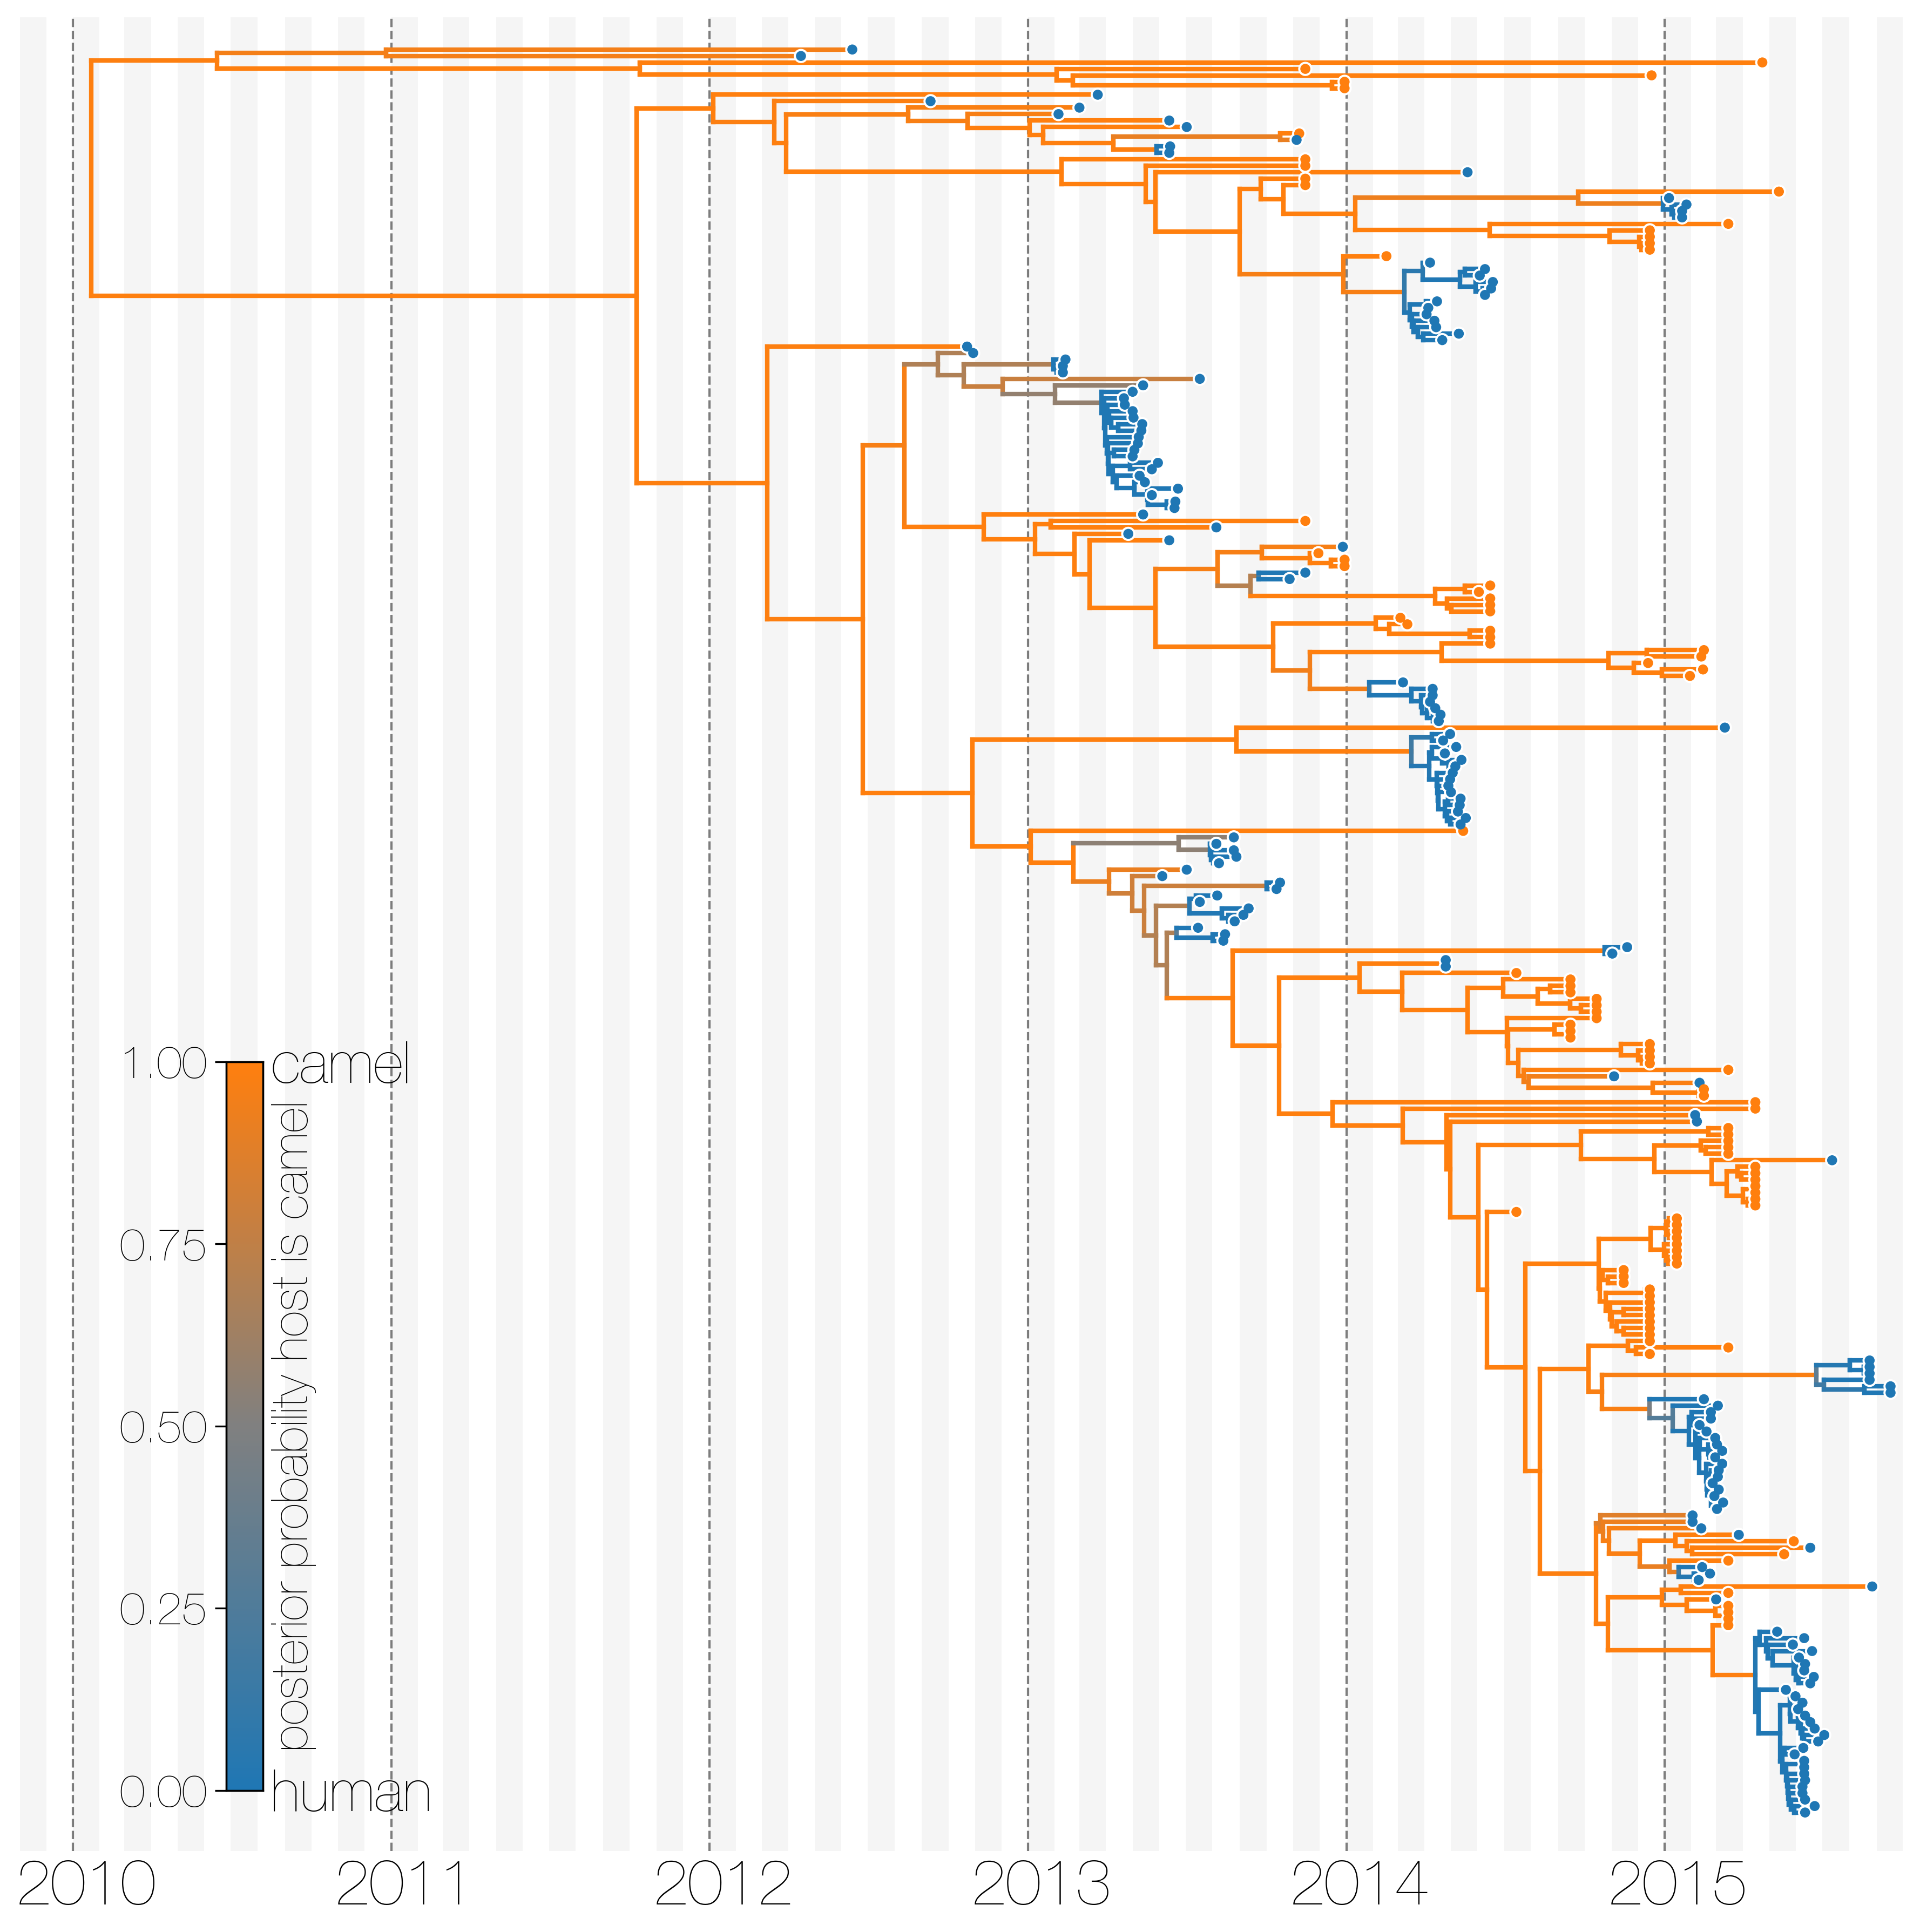
\includegraphics[width=0.65\textwidth]{figures/mers_mcc.png}
	\caption{\textbf{Typed maximum clade credibility tree of MERS-CoV sequences from humans and camels.}
	Maximum clade credibility (MCC) tree showing inferred ancestral hosts for MERS-CoV recovered using the structured coalescent.
	Vast majority of MERS-CoV evolution is inferred to occur in camels (orange) with human outbreaks (blue) representing evolutionary dead-ends for the virus.
	Whilst large clusters of human cases are apparent in the tree, significant contributions to human outbreaks are made by singleton sequences, likely representing recent cross-species transmissions that were caught early. 
	}
	\label{mcc}
\end{figure}

\subsection*{MERS epidemiology}
Although sequences in an outbreak necessarily represent a subset of all the cases, their clustering and resulting cluster sizes can be highly informative of underlying epidemiological processes that are otherwise inaccesible or unfeasible to study.
In our case we have used sequence data to disentangle the evolution of MERS-CoV into two discrete host compartments.
By removing the confounding effects of shared ancestry for MERS-CoV sequences we can treat every viral introduction into humans as an independent replicate of the transmission process in humans.


\section*{Discussion}

\subsection*{MERS-CoV in camels}
Our observation of recombinant MERS coronaviruses being transmitted to humans is not cause for concern by itself, however, the mere presence of detectable recombination implies that co-infection of camels with MERS-CoV is common.
By extension, frequent co-infection implies a high prevalence of the virus in camels, which is the main unsettling conclusion.
There is ample evidence for this from seroepidemiology, which has shown that XX\% of camels are infected by age XX.
Our results show that zoonotic transmission of MERS-CoV into humans is the main drivers for the continuation of the outbreak in the Arabian Peninsula. 
Prevalence of MERS-CoV in camels could easily be translated into force of infection and given the role of zoonotic transmission as the main driver for the outbreak only reiterates the importance of controlling the MERS coronavirus in the reservoir if the human side of the outbreak is to be brought under control.



\newpage

\section*{Methods}
\subsection*{Sequence data}
All MERS-CoV sequences were downloaded from GenBank.
Fragments of some strains submitted to GenBank as separate accessions were assembled into a single sequence.
Protein coding sequences were extracted and concatenated.
Sequences were annotated with available collection dates and hosts, designated as camel or human.
For partitioned analyses the alignment was split into two fragments, the first containing all nucleotides up to nucleotide 21000, and the rest of the genome being assigned to the second fragment.
Despite their divergence both Severe Acute Respiratory Syndrome (SARS) and MERS betacoronaviruses appear to recombine across position 21000, which may indicate the existence of a recombinogenic secondary RNA structure that remains to be described in its vicinity. %% "Work by Zhang et al. (66) suggested that the presence of a stable hairpin between two direct repeats increases the rate of homologous recombination in MLV. Their data led to the conclusion that stable secondary structures decrease processive RT synthesis and, further, that a functional NC can increase RT processivity. However, in this case, there were no corresponding in vitro data (such as primer extension assays) to correlate with the in vivo observations. Here, we have demonstrated for the first time a direct relationship between pausing in vitro and viral recombination in vivo."

\subsection*{Structured coalescent analyses}
MultiTypeTree module was used in BEAUti v2.4.3 to specify a structured coalescent model with two demes - humans and camels - based on GenBank records.
Analyses were run on codon position partitioned data with two separate HKY+$\Gamma_{4}$ nucleotide substitution models specified for codon positions 1+2 and 3.
A relaxed molecular clock with branch rates drawn from a lognormal distribution was used to infer the evolutionary rate from date calibrated tips.
Default priors were used for all parameters except for migration rates between demes for which an exponential prior with mean 1.0 was used.
An identical set up was used for analysing alignments split into two fragments, with independent clocks, trees and migration rates, but shared substitution models and deme population sizes.
Eight independent whole-genome MCMC analyses were run, for 200 million states each subsampling every 20000 states.
For two-fragment MCMC analyses ten independent runs were set up.
Due to the increased complexity of multitype tree parameter space 50\% of states from every analysis were discarded as burnin.

\subsection*{Epidemiological analyses}


\begin{equation}
r_{j} = \frac{\Gamma(kj+j-1)}{\Gamma(kj)\Gamma(j+1)} \frac{(\frac{R_{0}}{k})^{j-1}}{(1+\frac{R_{0}}{k})^{kj+j-1}}
\end{equation}

\subsection*{Data availability}


\section*{Acknowledgements}

\bibliographystyle{mbe.bst}
\bibliography{mers-structure}

\end{document}